\section{Introduction to Ask.fm}
\label{section:2.1}

Ask.fm is a social networking website that uses a question and answer format to allow its users to interact. Based in Riga, Latvia, the sites ease of access and the anonymity offered means that it is increasingly being used as a means to communicate abusive, bullying and sexualised content \cite{Webwise:2103}. A review of the Ask.fm ``Safety'' \cite{askfm_a:2014}, ``Privacy'' \cite{askfm_b:2014} and ``Terms'' \cite{askfm_c:2014} policy pages in November 2013 revealed the following worrying disclosures. Firstly it was stated that the content of the site was not monitored. The terms of service clearly stated that ``the ask.fm service allows for anonymous content which ask.fm does not monitor'' and that users of the site do so at their own risk. Secondly users were also warned in the terms of service that they may ``encounter content that may be deemed objectionable, obscene or in poor taste''.

Another review of the site in July 2014 showed a more user-friendly and potentially safer site where a list of unacceptable behaviours are given. Filters have been put in place for the detection of rude or offensive words \cite{askfm_d:2014}. Also given are a list of things to do and not to do in order to stay safe on the site and enjoy it \cite{askfm_e:2014}, a frequently asked questions and answers section for concerned parents \cite{askfm_f:2014} and better documented instructions on how to manage your user account and block users or anonymous questions \cite{askfm_g:2014}. Probably the most important change seen was the appointment of Annie Mullins OBE as Lead Advisor on User Safety at Ask.fm \cite{askfm_h:2014}. Ms Mullins, a member of the UK Home secretary's Task Force on Child Protection on the Internet received an OBE for services to children and young people.

The data from the Ask.fm site used in this research project was extracted from the site the weekend of Friday March 14, 2014 to Monday March 17, 2014.

The following pages give an overview of some of the main features of Ask.fm that a user of the site would use on a regular basis.

\subsection{Creating an Ask.fm Account}
To create an account the user need only provide some standard information such as user name, password, email address and date of birth(Figure \ref{fig:createaccount}).

\begin{figure}[h!]
	\centering
	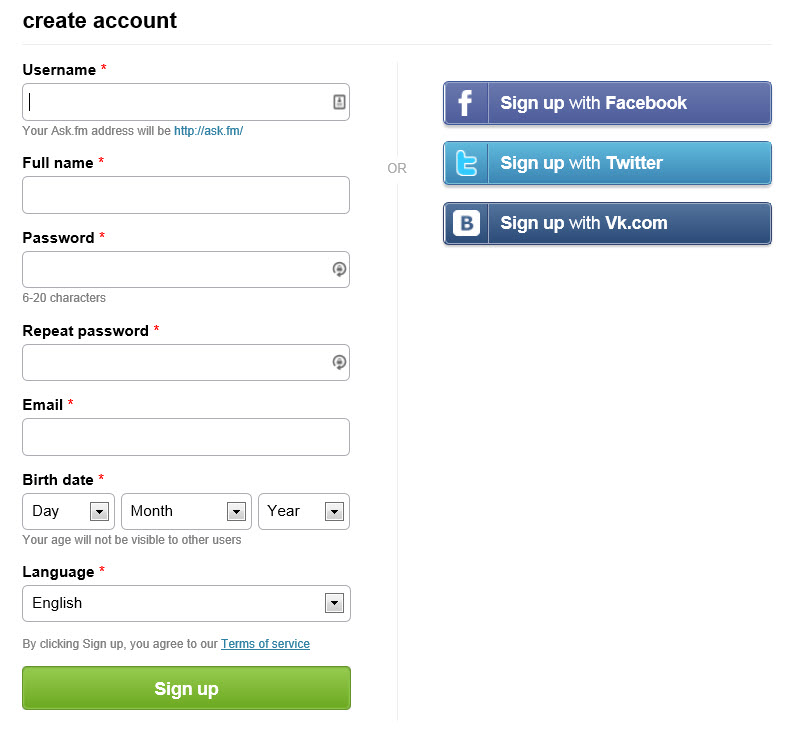
\includegraphics[scale=0.5]{Figures/Chapter2/CreateAccount.jpg}
	\caption{Creating an Ask.fm Account}
	\label{fig:createaccount}
\end{figure}

There is no obvious validation of the user details entered though an account can be linked to the users Facebook, Twitter or Vk.com accounts.

\subsection{Questions and Answers}
Any unanswered questions the user has will appear on their questions page (Figure \ref{fig:questions}). Users will always receive the question of the day and also have the option of receiving a random question if they have not received questions from other users.

\begin{figure}[h!]
	\centering
	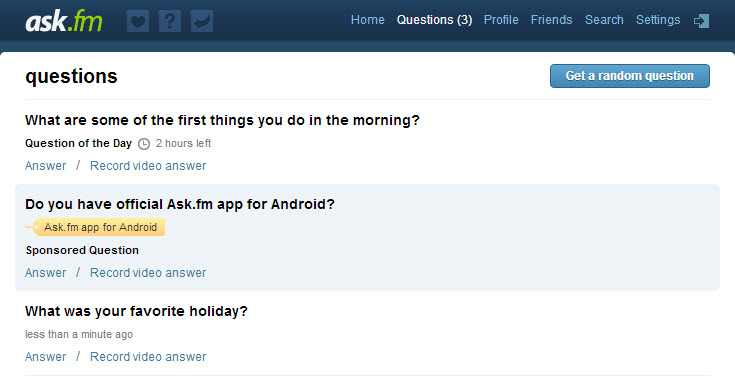
\includegraphics[scale=0.5]{Figures/Chapter2/Questions.jpg}
	\caption{Your Ask.fm Questions}
	\label{fig:questions}
\end{figure}

A question is a maximum of 300 characters long and a question can be asked whether the user has an Ask.fm account or not. Figure \ref{fig:askquestion_01} shows a question being asked by a user who is logged in and notice that the option to ask a question anonymously is also available. It is also possible to ask a question without having an account (Figure \ref{fig:askquestion_02}).

\begin{figure}[h!]
	\centering
	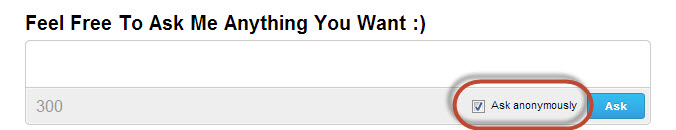
\includegraphics[scale=0.5]{Figures/Chapter2/AskQuestion_01.jpg}
	\caption{Asking a question when logged into your account}
	\label{fig:askquestion_01}
\end{figure}


\begin{figure}[h!]
	\centering
	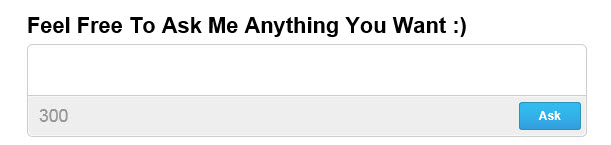
\includegraphics[scale=0.46]{Figures/Chapter2/AskQuestion_02.jpg}
	\caption{Asking a question when not logged into your account}
	\label{fig:askquestion_02}
\end{figure}

Text, a combination of text and a picture (Figure \ref{fig:answer}) or video can be used to answer the question.

\begin{figure}[h!]
	\centering
	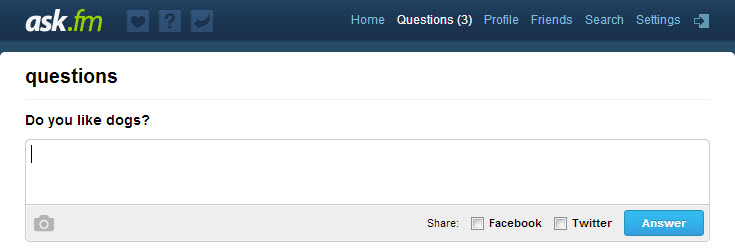
\includegraphics[scale=0.5]{Figures/Chapter2/Answer.jpg}
	\caption{Answering with text and an optional picture}
	\label{fig:answer}
\end{figure}

The option to share an answer using Twitter or Facebook is also available to the user.

\subsection{Privacy Setting, Reporting Abuse and Deleting Questions}
It should be highlighted that it is possible to prevent anonymous questions, to delete offensive questions before they are answered and also to report abuse.

To configure an Ask.fm account so that anonymous questions are not allowed a user can select the ``Do not allow anonymous questions'' on their Settings - Privacy page. On this privacy page it is also possible to select not to display answers on the Ask.fm stream (Figure \ref{fig:privacy}).

\begin{figure}[h!]
	\centering
	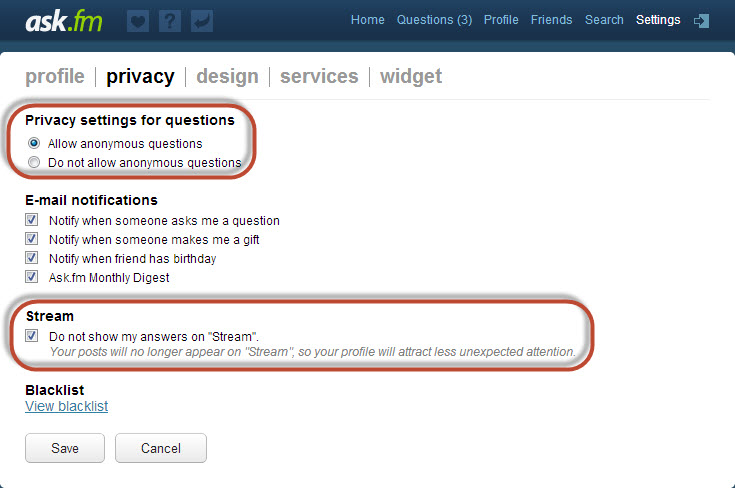
\includegraphics[scale=0.5]{Figures/Chapter2/PrivacySettings.jpg}
	\caption{Configuring privacy settings}
	\label{fig:privacy}
\end{figure}

Both users and questions/answers can be reported. In the top right-hand corner of each question there is a report flag. The option to report a user is available at the top of the users questions and answers page (Figure \ref{fig:report_01}). When the report button is clicked the type of inappropriate behaviour to report can be chosen (Figure \ref{fig:report_02}).

\begin{figure}[h!]
	\centering
	\includegraphics[scale=0.5]{Figures/Chapter2/report_01.jpg}
	\caption{Reporting a user or a question and answer}
	\label{fig:report_01}
\end{figure}


\begin{figure}[h!]
	\centering
	\includegraphics[scale=0.5]{Figures/Chapter2/report_02.jpg}
	\caption{Types of inappropriate behaviours to report}
	\label{fig:report_02}
\end{figure}

It is possible to delete a single question by hovering over the top right-hand side corner of the question where a delete ``X'' icon will appear (Figure \ref{fig:delete}). Alternatively, it is possible to delete all unanswered questions. Finally, it is also possible to block the asker of the question using the ``\textit{Block}'' icon. When a block is requested a new dialogue is displayed requesting the reason this user should be blocked (Figure \ref{fig:block}). This option is presented even when the user has posted anonymously. Blocking a user will cause unanswered question from this user to be deleted. 

\begin{figure}[h!]
	\centering
	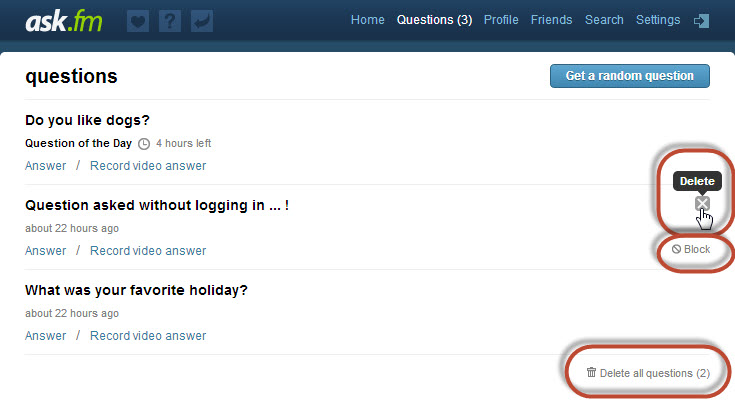
\includegraphics[scale=0.5]{Figures/Chapter2/DeleteQuestion.jpg}
	\caption{Deleting questions and blocking the user that asked the question}
	\label{fig:delete}
\end{figure}


\begin{figure}[h!]
	\centering
	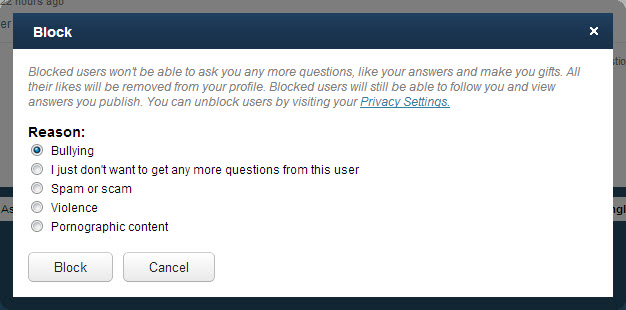
\includegraphics[scale=0.5]{Figures/Chapter2/Block.jpg}
	\caption{Blocking a user to prevent them asking further questions}
	\label{fig:block}
\end{figure}

\subsection{Deactivating an Account}
Finally, it is possible to deactivate an Ask.fm account from the users \textit{Settings - Profile} page but the account can be reactivated at any time.

\begin{figure}[h!]
	\centering
	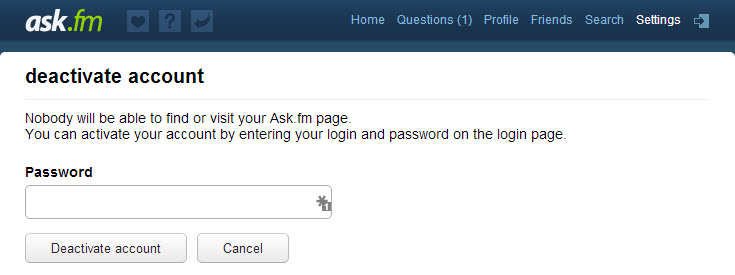
\includegraphics[scale=0.5]{Figures/Chapter2/Deactivate.jpg}
	\caption{Deactivating an account}
	\label{fig:deactivate}
\end{figure}